%**************************************%
%*    Generated from PreTeXt source   *%
%*    on 2019-06-25T21:10:36-06:00    *%
%*                                    *%
%*      https://pretextbook.org       *%
%*                                    *%
%**************************************%
\documentclass[twoside,11pt,]{book}
%% Custom Preamble Entries, early (use latex.preamble.early)
%% Default LaTeX packages
%%   1.  always employed (or nearly so) for some purpose, or
%%   2.  a stylewriter may assume their presence
\usepackage{geometry}
%% Some aspects of the preamble are conditional,
%% the LaTeX engine is one such determinant
\usepackage{ifthen}
%% etoolbox has a variety of modern conveniences
\usepackage{etoolbox}
\usepackage{ifxetex,ifluatex}
%% Raster graphics inclusion
\usepackage{graphicx}
%% Color support, xcolor package
%% Always loaded, for: add/delete text, author tools
%% Here, since tcolorbox loads tikz, and tikz loads xcolor
\PassOptionsToPackage{usenames,dvipsnames,svgnames,table}{xcolor}
\usepackage{xcolor}
%% Colored boxes, and much more, though mostly styling
%% skins library provides "enhanced" skin, employing tikzpicture
%% boxes may be configured as "breakable" or "unbreakable"
%% "raster" controls grids of boxes, aka side-by-side
\usepackage{tcolorbox}
\tcbuselibrary{skins}
\tcbuselibrary{breakable}
\tcbuselibrary{raster}
%% We load some "stock" tcolorbox styles that we use a lot
%% Placement here is provisional, there will be some color work also
%% First, black on white, no border, transparent, but no assumption about titles
\tcbset{ bwminimalstyle/.style={size=minimal, boxrule=-0.3pt, frame empty,
colback=white, colbacktitle=white, coltitle=black, opacityfill=0.0} }
%% Second, bold title, run-in to text/paragraph/heading
%% Space afterwards will be controlled by environment,
%% dependent of constructions of the tcb title
\tcbset{ runintitlestyle/.style={fonttitle=\normalfont\bfseries, attach title to upper} }
%% Spacing prior to each exercise, anywhere
\tcbset{ exercisespacingstyle/.style={before skip={1.5ex plus 0.5ex}} }
%% Spacing prior to each block
\tcbset{ blockspacingstyle/.style={before skip={2.0ex plus 0.5ex}} }
%% xparse allows the construction of more robust commands,
%% this is a necessity for isolating styling and behavior
%% The tcolorbox library of the same name loads the base library
\tcbuselibrary{xparse}
%% Hyperref should be here, but likes to be loaded late
%%
%% Inline math delimiters, \(, \), need to be robust
%% 2016-01-31:  latexrelease.sty  supersedes  fixltx2e.sty
%% If  latexrelease.sty  exists, bugfix is in kernel
%% If not, bugfix is in  fixltx2e.sty
%% See:  https://tug.org/TUGboat/tb36-3/tb114ltnews22.pdf
%% and read "Fewer fragile commands" in distribution's  latexchanges.pdf
\IfFileExists{latexrelease.sty}{}{\usepackage{fixltx2e}}
%% Text height identically 9 inches, text width varies on point size
%% See Bringhurst 2.1.1 on measure for recommendations
%% 75 characters per line (count spaces, punctuation) is target
%% which is the upper limit of Bringhurst's recommendations
\geometry{letterpaper,total={374pt,9.0in}}
%% Custom Page Layout Adjustments (use latex.geometry)
\geometry{papersize={7in,10in}, width=4.85in, inner=1in, height=8.5in, top=0.75in, twoside, ignoreheadfoot}
%% This LaTeX file may be compiled with pdflatex, xelatex, or lualatex executables
%% LuaTeX is not explicitly supported, but we do accept additions from knowledgeable users
%% The conditional below provides  pdflatex  specific configuration last
%% The following provides engine-specific capabilities
%% Generally, xelatex is necessary non-Western fonts
\ifthenelse{\boolean{xetex} \or \boolean{luatex}}{%
%% begin: xelatex and lualatex-specific configuration
\ifxetex\usepackage{xltxtra}\fi
%% realscripts is the only part of xltxtra relevant to lualatex 
\ifluatex\usepackage{realscripts}\fi
%% fontspec package provides extensive control of system fonts,
%% meaning *.otf (OpenType), and apparently *.ttf (TrueType)
%% that live *outside* your TeX/MF tree, and are controlled by your *system*
%% fontspec will make Latin Modern (lmodern) the default font
\usepackage{fontspec}
%% 
%% Extensive support for other languages
\usepackage{polyglossia}
%% Set main/default language based on pretext/@xml:lang value
%% document language code is "en-US", US English
%% usmax variant has extra hypenation
\setmainlanguage[variant=usmax]{english}
%% Enable secondary languages based on discovery of @xml:lang values
%% Enable fonts/scripts based on discovery of @xml:lang values
%% Western languages should be ably covered by Latin Modern Roman
%% end: xelatex and lualatex-specific configuration
}{%
%% begin: pdflatex-specific configuration
\usepackage[utf8]{inputenc}
%% PreTeXt will create a UTF-8 encoded file
%% begin: font setup and configuration for use with pdflatex
\usepackage{lmodern}
\usepackage[T1]{fontenc}
%% end: font setup and configuration for use with pdflatex
%% end: pdflatex-specific configuration
}
%% Monospace font: Inconsolata (zi4)
%% Sponsored by TUG: http://levien.com/type/myfonts/inconsolata.html
%% Loaded for documents with intentional objects requiring monospace
%% See package documentation for excellent instructions
%% One caveat, seem to need full file name to locate OTF files
%% Loads the "upquote" package as needed, so we don't have to
%% Upright quotes might come from the  textcomp  package, which we also use
%% We employ the shapely \ell to match Google Font version
%% pdflatex: "varqu" option produces best upright quotes
%% xelatex,lualatex: add StylisticSet 1 for shapely \ell
%% xelatex,lualatex: add StylisticSet 2 for plain zero
%% xelatex,lualatex: we add StylisticSet 3 for upright quotes
%% 
\ifthenelse{\boolean{xetex} \or \boolean{luatex}}{%
%% begin: xelatex and lualatex-specific monospace font
\usepackage{zi4}
\setmonofont[BoldFont=Inconsolatazi4-Bold.otf,StylisticSet={1,3}]{Inconsolatazi4-Regular.otf}
%% end: xelatex and lualatex-specific monospace font
}{%
%% begin: pdflatex-specific monospace font
%% "varqu" option provides textcomp \textquotedbl glyph
%% "varl"  option provides shapely "ell"
\usepackage[varqu,varl]{zi4}
%% end: pdflatex-specific monospace font
}
%% Symbols, align environment, bracket-matrix
\usepackage{amsmath}
\usepackage{amssymb}
%% allow page breaks within display mathematics anywhere
%% level 4 is maximally permissive
%% this is exactly the opposite of AMSmath package philosophy
%% there are per-display, and per-equation options to control this
%% split, aligned, gathered, and alignedat are not affected
\allowdisplaybreaks[4]
%% allow more columns to a matrix
%% can make this even bigger by overriding with  latex.preamble.late  processing option
\setcounter{MaxMatrixCols}{30}
%%
%%
%% Division Titles, and Page Headers/Footers
%% titlesec package, loading "titleps" package cooperatively
%% See code comments about the necessity and purpose of "explicit" option
\usepackage[explicit, pagestyles]{titlesec}
\newtitlemark{\chaptertitlename}
%% Set global/default page style for document due
%% to potential re-definitions after documentclass
\pagestyle{headings}
%%
%% Create globally-available macros to be provided for style writers
%% These are redefined for each occurence of each division
\newcommand{\divisionnameptx}{\relax}%
\newcommand{\titleptx}{\relax}%
\newcommand{\subtitleptx}{\relax}%
\newcommand{\shortitleptx}{\relax}%
\newcommand{\authorsptx}{\relax}%
\newcommand{\epigraphptx}{\relax}%
%% Create environments for possible occurences of each division
%% Environment for a PTX "chapter" at the level of a LaTeX "chapter"
\NewDocumentEnvironment{chapterptx}{mmmmmm}
{%
\renewcommand{\divisionnameptx}{Chapter}%
\renewcommand{\titleptx}{#1}%
\renewcommand{\subtitleptx}{#2}%
\renewcommand{\shortitleptx}{#3}%
\renewcommand{\authorsptx}{#4}%
\renewcommand{\epigraphptx}{#5}%
\chapter[#3]{#1}%
\label{#6}%
}{}%
%% Environment for a PTX "worksheet" at the level of a LaTeX "section"
\NewDocumentEnvironment{worksheet-section}{mmmmmm}
{%
\renewcommand{\divisionnameptx}{Worksheet}%
\renewcommand{\titleptx}{#1}%
\renewcommand{\subtitleptx}{#2}%
\renewcommand{\shortitleptx}{#3}%
\renewcommand{\authorsptx}{#4}%
\renewcommand{\epigraphptx}{#5}%
\section[#3]{#1}%
\label{#6}%
}{}%
%% Environment for a PTX "worksheet" at the level of a LaTeX "section"
\NewDocumentEnvironment{worksheet-section-numberless}{mmmmmm}
{%
\renewcommand{\divisionnameptx}{Worksheet}%
\renewcommand{\titleptx}{#1}%
\renewcommand{\subtitleptx}{#2}%
\renewcommand{\shortitleptx}{#3}%
\renewcommand{\authorsptx}{#4}%
\renewcommand{\epigraphptx}{#5}%
\section*{#1}%
\addcontentsline{toc}{section}{#3}
\label{#6}%
}{}%
%%
%% Styles for six traditional LaTeX divisions
\titleformat{\chapter}[display]
{\normalfont\huge\bfseries}{\divisionnameptx\space\thechapter}{20pt}{\Huge#1}
[{\Large\authorsptx}]
\titleformat{name=\chapter,numberless}[display]
{\normalfont\huge\bfseries}{}{0pt}{#1}
[{\Large\authorsptx}]
\titlespacing*{\chapter}{0pt}{50pt}{40pt}
\titleformat{\section}[hang]
{\normalfont\Large\bfseries}{\thesection}{1ex}{#1}
[{\large\authorsptx}]
\titleformat{name=\section,numberless}[block]
{\normalfont\Large\bfseries}{}{0pt}{#1}
[{\large\authorsptx}]
\titlespacing*{\section}{0pt}{3.5ex plus 1ex minus .2ex}{2.3ex plus .2ex}
\titleformat{\subsection}[hang]
{\normalfont\large\bfseries}{\thesubsection}{1ex}{#1}
[{\normalsize\authorsptx}]
\titleformat{name=\subsection,numberless}[block]
{\normalfont\large\bfseries}{}{0pt}{#1}
[{\normalsize\authorsptx}]
\titlespacing*{\subsection}{0pt}{3.25ex plus 1ex minus .2ex}{1.5ex plus .2ex}
\titleformat{\subsubsection}[hang]
{\normalfont\normalsize\bfseries}{\thesubsubsection}{1em}{#1}
[{\small\authorsptx}]
\titleformat{name=\subsubsection,numberless}[block]
{\normalfont\normalsize\bfseries}{}{0pt}{#1}
[{\normalsize\authorsptx}]
\titlespacing*{\subsubsection}{0pt}{3.25ex plus 1ex minus .2ex}{1.5ex plus .2ex}
\titleformat{\paragraph}[hang]
{\normalfont\normalsize\bfseries}{\theparagraph}{1em}{#1}
[{\small\authorsptx}]
\titleformat{name=\paragraph,numberless}[block]
{\normalfont\normalsize\bfseries}{}{0pt}{#1}
[{\normalsize\authorsptx}]
\titlespacing*{\paragraph}{0pt}{3.25ex plus 1ex minus .2ex}{1.5em}
%%
%% Semantic Macros
%% To preserve meaning in a LaTeX file
%%
%% \mono macro for content of "c", "cd", "tag", etc elements
%% Also used automatically in other constructions
%% Simply an alias for \texttt
%% Always defined, even if there is no need, or if a specific tt font is not loaded
\newcommand{\mono}[1]{\texttt{#1}}
%%
%% Following semantic macros are only defined here if their
%% use is required only in this specific document
%%
%% Division Numbering: Chapters, Sections, Subsections, etc
%% Division numbers may be turned off at some level ("depth")
%% A section *always* has depth 1, contrary to us counting from the document root
%% The latex default is 3.  If a larger number is present here, then
%% removing this command may make some cross-references ambiguous
%% The precursor variable $numbering-maxlevel is checked for consistency in the common XSL file
\setcounter{secnumdepth}{1}
%% begin: General AMS environment setup
%% Environments built with amsthm package
\usepackage{amsthm}
%% Numbering for Theorems, Conjectures, Examples, Figures, etc
%% Controlled by  numbering.theorems.level  processing parameter
%% Numbering: all theorem-like numbered consecutively
%% i.e. Corollary 4.3 follows Theorem 4.2
%% Always need some theorem environment to set base numbering scheme
%% even if document has no theorems (but has other environments)
%% Create a never-used style first, always
%% simply to provide a global counter to use, namely "cthm"
\newtheorem{cthm}{BadTheoremStringName}[section]
%% AMS "proof" environment is not used, but we leave previously
%% implemented \qedhere in place, should the LaTeX be recycled
\renewcommand{\qedhere}{\relax}
%% end: General AMS environment setup
%%
%% xparse environments for introductions and conclusions of divisions
%%
%% introduction: in a structured division
\NewDocumentEnvironment{introduction}{m}
{\notblank{#1}{\noindent\textbf{#1}\space}{}}{\par\medskip}
%% Divisional exercises (and worksheet) as LaTeX environments
%% Third argument is option for extra workspace in worksheets
%% Hanging indent occupies a 5ex width slot prior to left margin
%% Experimentally this seems just barely sufficient for a bold "888."
%% Division exercises, not in exercise group
\tcbset{ divisionexercisestyle/.style={bwminimalstyle, runintitlestyle, exercisespacingstyle, left=5ex, breakable, parbox=false } }
\newtcolorbox{divisionexercise}[4]{divisionexercisestyle, before title={\hspace{-5ex}\makebox[5ex][l]{#1.}}, title={\notblank{#2}{#2\space}{}}, phantom={\hypertarget{#4}{}}, after={\notblank{#3}{\newline\rule{\workspacestrutwidth}{#3\textheight}\newline}{}}}
%% Worksheet exercises may have workspaces
\newlength{\workspacestrutwidth}
%% @workspace strut is invisible
\setlength{\workspacestrutwidth}{0pt}
%% Localize LaTeX supplied names (possibly none)
\renewcommand*{\chaptername}{Chapter}
\setcounter{chapter}{-1}
%% "tcolorbox" environment for a single image, occupying entire \linewidth
%% arguments are left-margin, width, right-margin, as multiples of
%% \linewidth, and are guaranteed to be positive and sum to 1.0
\tcbset{ imagestyle/.style={bwminimalstyle} }
\NewTColorBox{image}{mmm}{imagestyle,left skip=#1\linewidth,width=#2\linewidth}
%% Figures, Tables, Listings, Named Lists, Floats
%% The [H]ere option of the float package fixes floats in-place,
%% in deference to web usage, where floats are totally irrelevant
%% You can remove some of this setup, to restore standard LaTeX behavior
%% HOWEVER, numbering of figures/tables AND theorems/examples/remarks, etc
%% may de-synchronize with the numbering in the HTML version
%% You can remove the "placement={H}" option to allow flotation and
%% preserve numbering, BUT the numbering may then appear "out-of-order"
%% Floating environments: http://tex.stackexchange.com/questions/95631/
\usepackage{float}
\usepackage{newfloat}
\usepackage{caption}%% Adjust stock figure environment so that it no longer floats
\SetupFloatingEnvironment{figure}{fileext=lof,placement={H},within=section,name=Figure}
\captionsetup[figure]{labelfont=bf}
%% http://tex.stackexchange.com/questions/16195
\makeatletter
\let\c@figure\c@cthm
\makeatother
%% More flexible list management, esp. for references
%% But also for specifying labels (i.e. custom order) on nested lists
\usepackage{enumitem}
%% hyperref driver does not need to be specified, it will be detected
%% Footnote marks in tcolorbox have broken linking under
%% hyperref, so it is necessary to turn off all linking
%% It *must* be given as a package option, not with \hypersetup
\usepackage[hyperfootnotes=false]{hyperref}
%% configure hyperref's  \url  to match listings' inline verbatim
\renewcommand\UrlFont{\small\ttfamily}
%% Hyperlinking active in electronic PDFs, all links solid and blue
\hypersetup{colorlinks=true,linkcolor=blue,citecolor=blue,filecolor=blue,urlcolor=blue}
\hypersetup{pdftitle={Mathematics for Elementary Teachers}}
%% If you manually remove hyperref, leave in this next command
\providecommand\phantomsection{}
%% Graphics Preamble Entries
\usepackage{tikz, pgfplots}
\usetikzlibrary{positioning,matrix,arrows}
\usetikzlibrary{shapes,decorations,shadows,fadings,patterns}
\usetikzlibrary{decorations.markings}
%% If tikz has been loaded, replace ampersand with \amp macro
%% Custom Preamble Entries, late (use latex.preamble.late)
%% Begin: Author-provided packages
%% (From  docinfo/latex-preamble/package  elements)
%% End: Author-provided packages
%% Begin: Author-provided macros
%% (From  docinfo/macros  element)
%% Plus three from MBX for XML characters
\newcommand{\N}{\mathbb N}
\newcommand{\Z}{\mathbb Z}
\newcommand{\Q}{\mathbb Q}
\newcommand{\R}{\mathbb R}
\newcommand{\C}{\mathbb C}
\newcommand{\inv}{^{-1}}
\newcommand{\st}{:}
\renewcommand{\iff}{\leftrightarrow}
\newcommand{\Iff}{\Leftrightarrow}
\newcommand{\imp}{\rightarrow}
\newcommand{\Imp}{\Rightarrow}
\newcommand{\isom}{\cong}

\renewcommand{\bar}{\overline}
\newcommand{\card}[1]{\left| #1 \right|}
\newcommand{\lt}{<}
\newcommand{\gt}{>}
\newcommand{\amp}{&}
%% End: Author-provided macros
\begin{document}
\frontmatter
%% begin: half-title
\thispagestyle{empty}
{\centering
\vspace*{0.28\textheight}
{\Huge Mathematics for Elementary Teachers}\\[2\baselineskip]
{\LARGE A Workbook}\\
}
\clearpage
%% end:   half-title
%% begin: adcard
\thispagestyle{empty}
\null%
\clearpage
%% end:   adcard
%% begin: title page
%% Inspired by Peter Wilson's "titleDB" in "titlepages" CTAN package
\thispagestyle{empty}
{\centering
\vspace*{0.14\textheight}
%% Target for xref to top-level element is ToC
\addtocontents{toc}{\protect\hypertarget{book-376575413712}{}}
{\Huge Mathematics for Elementary Teachers}\\[\baselineskip]
{\LARGE A Workbook}\\[3\baselineskip]
{\Large \textbraceleft{}author\textbraceright{}}\\[0.5\baselineskip]
{\Large \textbraceleft{}institution\textbraceright{}}\\[3\baselineskip]
{\Large June 25, 2019}\\}
\clearpage
%% end:   title page
%% begin: copyright-page
\thispagestyle{empty}
\hypertarget{colophon-376568827296}{}\vspace*{\stretch{2}}
\noindent{\bfseries Website}: \href{[website]}{\mono{[website]}}\par\medskip
\noindent\textcopyright{}[copyright-year]\quad{}[copyright-holder]\\[0.5\baselineskip]
 This work is licensed under the Creative Commons Attribution-ShareAlike 4.0 International License. To view a copy of this license, visit \href{http://creativecommons.org/licenses/by-sa/4.0/}{http:\slash{}\slash{}creativecommons.org\slash{}licenses\slash{}by-sa\slash{}4.0\slash{}}\par\medskip
\vspace*{\stretch{1}}
\null\clearpage
%% end:   copyright-page
%% begin: table of contents
%% Adjust Table of Contents
\setcounter{tocdepth}{2}
\renewcommand*\contentsname{Contents}
\tableofcontents
%% end:   table of contents
\mainmatter
%
%
\typeout{************************************************}
\typeout{Chapter 0 Worksheets}
\typeout{************************************************}
%
\begin{chapterptx}{Worksheets}{}{Worksheets}{}{}{chapter-376568651552}
%
%
\typeout{************************************************}
\typeout{Worksheet 0 Addition and Subtraction Problems with Strip (Tape) Diagrams}
\typeout{************************************************}
%
\newgeometry{left=1.25cm, right=1.25cm, top=1.25cm, bottom=1.25cm}
\begin{worksheet-section-numberless}{Addition and Subtraction Problems with Strip (Tape) Diagrams}{}{Addition and Subtraction Problems with Strip (Tape) Diagrams}{}{}{worksheet-376575402448}
\begin{introduction}{}%
\hypertarget{p-376568959280}{}%
Directions: For each problem create strip (tape) diagram(s) to model the situation.  Also write an equation that models the situation.  Be sure that your equation matches the actual actions in the story problem, not just how you’d solve it.%
\end{introduction}%
\begin{divisionexercise}{1}{}{0.1}{exercise-376568905264}%
\hypertarget{p-376568904528}{}%
Rachel had 17 CDs.  After she got some more CDs, she had 43 CDs.  How many CDs did Rachel get?%
\end{divisionexercise}%
\begin{divisionexercise}{2}{}{0.1}{exercise-376568967376}%
\hypertarget{p-376568966640}{}%
Rachel had 43 CDs.  After she gave some away, she had 17 CDs left.  How many did she give away?%
\end{divisionexercise}%
\begin{divisionexercise}{3}{}{0.1}{exercise-376568970656}%
\hypertarget{p-376568970016}{}%
Rachel had some CDs.  After she gave 26 away, she had 17 left.  How many CDs did Rachel have at the start?%
\end{divisionexercise}%
\begin{divisionexercise}{4}{}{0.1}{exercise-376568969248}%
\hypertarget{p-376568973808}{}%
Rachel has 43 CDs.  If 26 are hip hop and the rest are rap, how many rap CDs does she have?%
\end{divisionexercise}%
\begin{divisionexercise}{5}{}{0.1}{exercise-376568973056}%
\hypertarget{p-376568972320}{}%
Rachel has 43 CDs.  Benny has 26 CDs.  How many more CDs does Rachel have than Benny?%
\end{divisionexercise}%
\begin{divisionexercise}{6}{}{0.1}{exercise-376541741248}%
\hypertarget{p-376541740608}{}%
Benny has 26 CDs. Benny has 17 fewer CDs than Rachel.  How many CDs does Rachel have?%
\end{divisionexercise}%
\begin{divisionexercise}{7}{}{0.1}{exercise-376541739856}%
\hypertarget{p-376541739120}{}%
Rachel has 43 CDs. Rachel has 17 more CDs than Benny.  How many CDs does Benny have?%
\end{divisionexercise}%
\end{worksheet-section-numberless}
\restoregeometry
%
%
\typeout{************************************************}
\typeout{Worksheet 0 Reasoning with Addition and Subtraction Scenarios}
\typeout{************************************************}
%
\newgeometry{left=1.25cm, right=1.25cm, top=1.25cm, bottom=1.25cm}
\begin{worksheet-section-numberless}{Reasoning with Addition and Subtraction Scenarios}{}{Reasoning with Addition and Subtraction Scenarios}{}{}{worksheet-376568941824}
\begin{divisionexercise}{1}{}{0.1}{exercise-376568960288}%
\hypertarget{p-376541731568}{}%
1.	John and Anne want to calculate \textdollar{}37-\textdollar{}19 by first calculating%
\begin{equation*}
\$37-\$20=\$17 
\end{equation*}
John says they must now subtract the \textdollar{}1 remaining from \textdollar{}17, while Anne says they must add it.  Who is correct?  Use two different models (e.g., number line and strip diagram) to represent this scenario to make it clear who is correct.%
\end{divisionexercise}%
\begin{divisionexercise}{2}{}{0.1}{exercise-376541730288}%
\hypertarget{p-376541729648}{}%
John and Anne want to calculate \textdollar{}3.94 -\textdollar{}1.97 by first calculating%
\begin{equation*}
\$3.97-\$1.97 = \$2 
\end{equation*}
John says in this case they also need to subtract the \textdollar{}0.03 remaining from \textdollar{}2, while Anne says they must add it.  Who is correct?  Use two different models (e.g., number line and strip diagram) to represent this scenario to make it clear who is correct.%
\end{divisionexercise}%
\begin{divisionexercise}{3}{}{0.1}{exercise-376541728352}%
\hypertarget{p-376541727616}{}%
Jamirez says he can calculate \textdollar{}3.74 -\textdollar{}1.97 by first adding \textdollar{}0.03 to each number and calculating \textdollar{}3.77-\textdollar{}2 instead.  How could we use a model\slash{}diagram to show that Jamirez’s method is also valid?%
\end{divisionexercise}%
\begin{divisionexercise}{4}{}{0.1}{exercise-376541726752}%
\hypertarget{p-376541726016}{}%
Jon’s time for running a lap in gym class is 1.4 minutes.  Jacky’s time is 1.32 minutes.  Jon thinks that he’s faster than Jacky since 4 is less than 32 so 1.4 must be less than 1.32.  Is Jon correct?  How we could convince the students whose time is faster and by how much?%
\end{divisionexercise}%
\begin{divisionexercise}{5}{}{0.1}{exercise-376541725072}%
\hypertarget{p-376541724336}{}%
A local park’s program committee is raising money by holding mountain bike races on a course through the local park.  During each race, a computer tracks the competitors’ locations on the course using GPS tracking.  The table below shows how far each competitor is from a checkpoint.%
\begin{image}{0}{1}{0}%
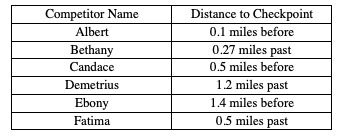
\includegraphics[width=1\linewidth]{images/reasoning-table-checkpoint.png}
\end{image}%
\leavevmode%
\begin{enumerate}[label=(\alph*)]
\item\hypertarget{li-376541722688}{}The checkpoint is represented by 0 on the number line below.  Locate and label points on the number line for the positions of each listed participant. \begin{image}{0}{1}{0}%
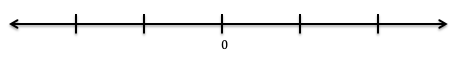
\includegraphics[width=1\linewidth]{images/blank-number-line.png}
\end{image}%
%
\item\hypertarget{li-376541721648}{}Which competitor is closest to the checkpoint?%
\item\hypertarget{li-376541721264}{}Two competitors are the same distance from the checkpoint.  Are they in the same location?  Explain.%
\item\hypertarget{li-376541720752}{}Who is closer to finishing the race – Bethany or Candace?%
\end{enumerate}
\end{divisionexercise}%
\begin{divisionexercise}{6}{}{0.1}{exercise-376541719984}%
\hypertarget{p-376541719248}{}%
Andrea and Marta are testing three different coolers to see which keeps the temperature the coolest.  They placed a bag of ice in each cooler, and then measured the air temperature inside each cooler after 90 minutes.  The temperatures are recorded below:%
\begin{image}{0}{1}{0}%
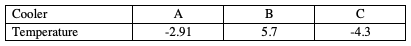
\includegraphics[width=1\linewidth]{images/reasoning-table-cooler.png}
\end{image}%
\hypertarget{p-376541718112}{}%
Marta wrote the following inequality: -4.3 = -2.91 = 5.7 Andrea said Marta made a mistake, and that the inequality should be: -2.91 = -4.3 = 5.7%
\par
\hypertarget{p-376541717552}{}%
Is either student correct?  Explain.  Use a number line to help justify your answer.  What misconceptions might the student(s) have had that caused the incorrect inequality?%
\end{divisionexercise}%
\end{worksheet-section-numberless}
\restoregeometry
\end{chapterptx}
\end{document}